%The \introduction command is provided as a convenience.
%if you want special chapter formatting, you'll probably want to avoid using it altogether
		\setcounter{secnumdepth}{0}
\chapter*{Introduction}
    \addcontentsline{toc}{chapter}{Introduction}
		\chaptermark{Introduction}
		\markboth{Introduction}{Introduction}

% The three lines above are to make sure that the headers are right, that the intro gets included in the table of contents, and that it doesn't get numbered 1 so that chapter one is 1.
\epigraph{ I am an old man now, and when I die and go to heaven, there are two matters on which I hope for enlightenment. One is quantum electrodynamics, and the other is the turbulent motion of fluids. And about the former, I am optimistic}{Horace Lamb, 1932}
	
The turbulence problem can be stated simply -- Is there a predictive model for the development of the internal structures of turbulent flows? In this case it is deceptively simple, for much like a small, unnamed village in coastal Armorica holding out against the Romans, the turbulence problem that has confounded physicists and engineers for centuries. Understanding turbulence is vitally important, since turbulent flows appear in artificial scenarios such as the flow around ships or aircraft, and in natural scenarios from the atmosphere of Jupiter to the blood flow in the heart.  Turbulent flows are typically characterized by the {\bf Reynolds number}, which is the (dimensionless) ratio between the inertial and viscous damping forces. At small \ReN, viscosity dominates, and smooths out large velocity gradients in the fluid, resulting in the well-ordered {\bf laminar} flow. At large \ReN, kinetic energy is dissipated at a lower rate, allowing for the existence of increasingly complex flow structures, such as eddies or vortices, which are characteristic of turbulence.  
\begin{figure}[h]
\centerline{
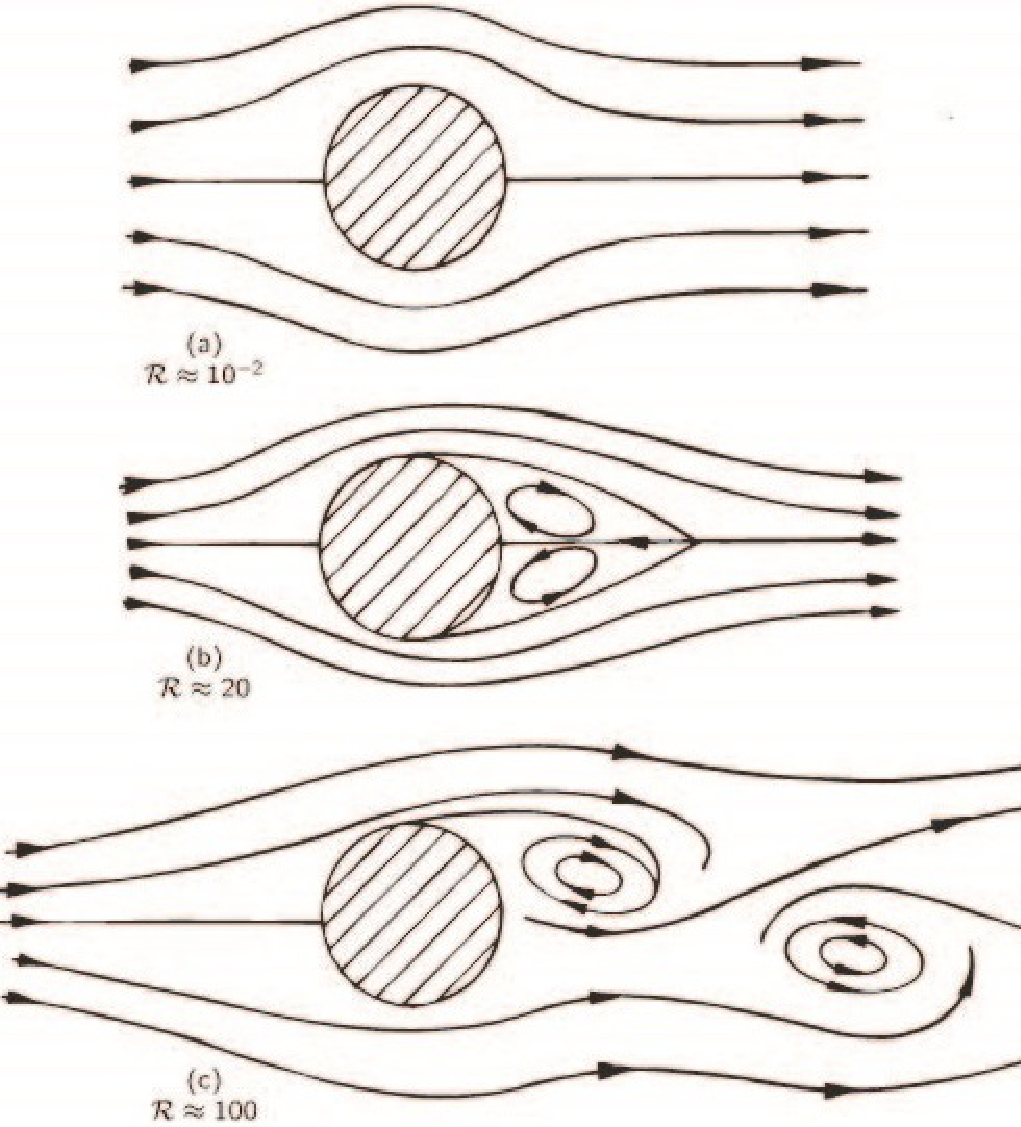
\includegraphics[scale=0.4]{Figs/CylinderReFlow}}
\caption{Representations of cylinder wakes at various \ReN. Notice that the flow goes from laminar in (a) to turbulent in (c), with two prominent vorticies. Reproduced from the Feynman Lectures on Physics, Chapter 41.}\label{fig:cylinderWake}
\end{figure}

\section{Transition to Turbulence}

From the definition of the Reynolds number, it is clear that in the limit of $\ReN \rightarrow 0$, the only steady state solution is the laminar flow state, while in the limit $\ReN \rightarrow \infty$, turbulent flow states can also exist. It might therefore be reasonable to expect that as \ReN~increases, the flow should become steadily more turbulent. However, experiments in Taylor-Couette and pipe flows, among others, indicate that turbulence develops suddenly at some critical value of \ReN. There are in general two routes by which systems transition to turbulence. In the supercritical transition, an increase in \ReN~above some critical value results in the loss of global stability of the laminar state\footnote{That is to say, it is no longer stable against perturbations of any amplitude} and the emergence of new stable solutions of higher complexity, which eventually bifurcate into even more complex states at higher critical values, eventually resulting in turbulence. Supercritical transitions occur in Taylor-Couette flow with low outer-cylinder rotation rates, and well as in Rayleigh-Bernard convection. \\

The second, more complex transition is the subcritical transition. In the subcritical transition, the laminar state loses global stability at lower \ReN~than linear stability analysis would predict, and the flow transitions \emph{directly} to turbulence, instead of increasingly steadily in complexity. Since they are not well predicted by linear stability analysis, subcritical transitions are less well understood, but nevertheless can be physically important. Subcritical transitions occur in pressure-driven flows in pipes, which models flows such as those in hypodermic needles or lung alveoli, or shear-driven flow between two infinite parallel plates (displayed in \refFig{fig:planeCouette}), which is known as plane Couette flow, and is the focus of this thesis \rf{Eckhardt2008,Manneville2015}.
\begin{figure}
\centerline{
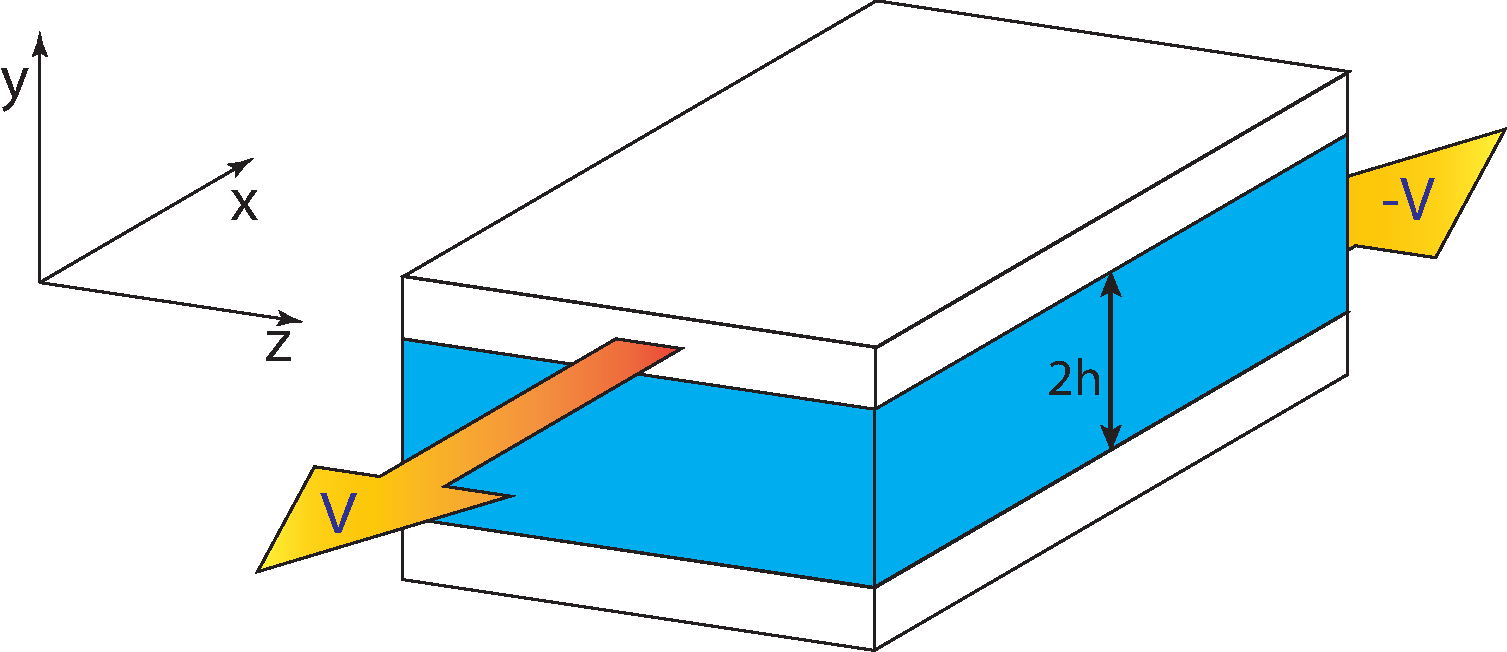
\includegraphics[scale=0.4]{Figs/planeCouetteDiagram}}
\caption{A diagram of the plane Couette geometry. The upper and lower plates extend infinitely in the plane, as does the fluid filling the gap.}\label{fig:planeCouette}
\end{figure}

\section{Plane Couette Flow} 

The geometry of the full plane Couette system is extremely simple, with only one geometrical parameter $h$, the half-distance between the parallel plates, and one kinematic parameter $V$, the velocity of the upper plate\footnote{While in principle the upper and lower plate can have different velocities, there should always be a reference frame in which the upper plate has velocity $V$, and the lower plate has velocity $-V$.}, giving the Reynolds number as 
\begin{equation}
\ReN = \frac{hV}{\nu},
\end{equation}
where $\nu$ is the kinematic viscosity. When \ReN~is very small, only the laminar flow state is stable, which in the case of plane Couette flow is given by the linear velocity profile shown in \refFig{fig:planeCouetteBulk}. As \ReN~increases, however, we would expect the emergence of long lived turbulence, which has been seen in experiments \rf{Daviaud1992}.
\begin{figure}
\centerline{
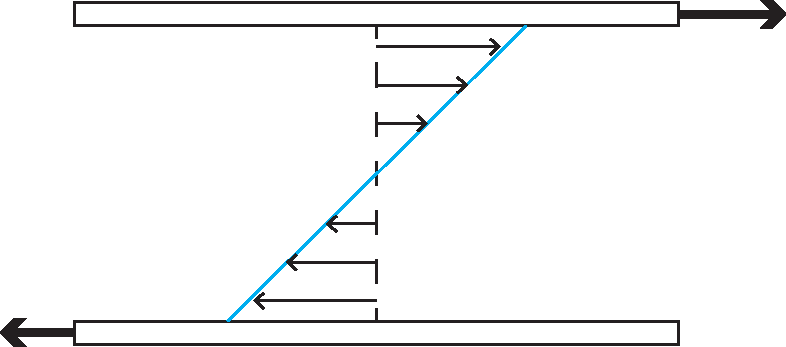
\includegraphics[scale=0.6]{Figs/planeCouetteMeanFlow}}
\caption{A cross-sectional representation of plane Couette flow, with the laminar velocity profile shown. By symmetry, the laminar profile must be the same everywhere.}\label{fig:planeCouetteBulk}
\end{figure}

\section{Tackling Turbulence} 

The traditional approach towards the analysis of turbulence for the last century has been the statistical approach initially developed by Reynolds, Prandtl, von Karman, Kolmogorov and others\rf{Pope2000}. At the core of the statistical approach to turbulence is the assumption that turbulent flow states can be expressed as random perturbations around some mean flow. At extremely high \ReN, where direct numerical simulation (DNS) of the flow is computationally infeasible, the statistical approach is invaluable, but at low-to-moderate \ReN, these models can become less accurate -- for example, Reynolds stress models have no \ReN~dependence, but DNS shows that there are \ReN-dependent effects. Even ignoring the moderate \ReN behavior of the statistical models, the fundamental issue with the statistical approach is its discarding of the dynamical information about turbulence. Methods like RANS time average the perturbations away, while LES explicitly does not resolve small scale structures, and thus cannot truly provide an answer to the turbulence problem. \\

An alternate approach was proposed by Eberhard Hopf in 1948. Hopf suggested that solutions to the Navier-Stokes equations might be thought of as trajectories in an infinite dimensional state space in which each point corresponded to a possible velocity field. To better understand what this would mean, consider the velocity field at a point in the fluid, pictured in \refFig{fig:VectorSpace}. In order to describe the velocity vector, three numbers are required (each of which can take any real value), so this microsystem has three dimensions. Now any finite fluid volume will have an uncountably infinite number of points at which the velocity field has a value, so we would need an uncountably infinite set of numbers to describe any velocity field, which would then reside in an infinite dimensional vector space.
\begin{figure}
\centerline{
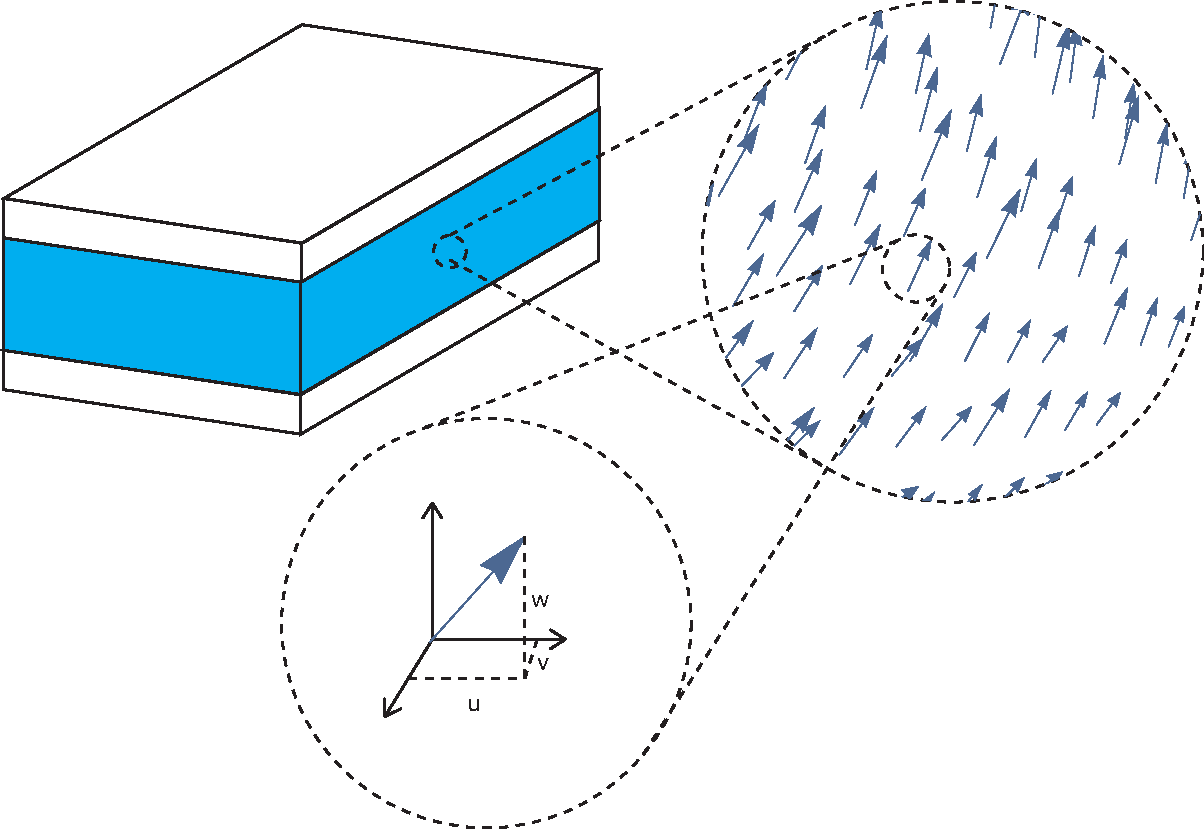
\includegraphics[scale=0.6]{Figs/VectorSpace}}
\caption{At each point in the fluid volume, the velocity field has a value that is described by three numbers, thus requiring three dimensions to track over time.}\label{fig:VectorSpace}
\end{figure}
Luckily, every point in the space does not necessarily corrspond to a solution of the Navier-Stokes equation; for finite \ReN, for instance, the gradient of the velocity field cannot be too large. Hopf thus conjectured that physical trajectories, corresponding to solutions to the Navier-Stokes equation would lie on some finite-dimensional manifold (known as the {\bf inertial manifold}) embedded within this infinite dimensional space. This transition of an inertial manifold from infinite to finite dimensional spaces by varying a control parameter has been rigorously deomonstrated under certain conditions\rf{Foias1988}. For the Navier-Stokes equation, the inertial manifold's control parameter is \ReN, and physical intiuition suggests that its structure should also have \ReN~dependence, since at very low \ReN, the only physical solution is the laminar state, and as \ReN~increases, more complex flows become physically permissible. Hopf proposed finally that turbulence in this view was simply a trajectory that would travel across wide distances on the manifold. \\

Unfortunately for Hopf, the computer power necessary to pursue this line of work was not available in 1948, leading him to comment in frustration that ``“the great mathematical difficulties of these important problems are well
known and at present the way to a successful attack on them seems hopelessly
barred". It would take until 1963 and the derivation of the Lorenz attractor for the first numerical state-space analysis of turbulence\rf{Lorenz1963}, albeit for a highly truncated version of Navier-Stokes, designed to investigate Rayleigh-Bernard convection. There have also been a number of efforts to explore the tructure of invariant manifolds in moderate turbulence Navier-Stokes, such as Proper Orthogonal Decomposition\rf{Aubry1988} and the `self-sustaining process theory'\rf{Dauchot2000}, but while fruitful they are nevertheless models of turbulent flow, and not an exact analysis of Navier-Stokes. Another avenue of research emerged in 1990, when Nagata computed nontrivial equilibirum flow states in plane Couette flow by continuing the wave vortex solution of Taylor-Couette flow\rf{Nagata1990}. This class of solutions, which were named {\bf exact coherent structures} by Waleffe\rf{Waleffe2001} are the result of calculating exact, invariant solutions of the fully resolved Navier-Stokes equation. The family of \ecs~was expanded with the discovery of travelling wave equilibira by Nagata in 1997, the computation of periodic orbits by Kawahara and Kida in 2001\rf{Kawahara2001}, and the computation of \emph{relative} periodic orbits\footnote{That is, flow states that are periodic after some phase shift} by Viswanath in 2007\rf{Viswanath2007}. The ultimate hope of this line of research is that turbulence can be viewed as chaotic trajectories on the inertial manifold that are guided by \ecs~(\refFig{fig:guidedTurbulence}), implying that a fundamental understanding of \ecs~would lead to a better understanding of turbulent dynamics. \\
\begin{figure}
\centerline{
\includegraphics[scale=0.8]{Figs/phaseSpaceTraj}}
\caption{A turbulent trajectory in black appears chaotic in isolation, but is in fact guided by \ecs~of the flow}\label{fig:guidedTurbulence}
\end{figure}

While there has been a great deal of progess in this field, much of it has been computational, though experiments by Hof and de Lozar are at present the only direct experimental verifications for the existence of \ecs~in nature. However, indirect results, such as the resemblence of the upper branch solution to the roll-streak structure seen in DNS\rf{Gibson2008}, and the potential role of the stable manifold of the lower branch solution in separating the turbulent and laminar basins of attraction suggest that \ecs likely play a fundamental role in the behavior and evolution of turbulent flow states. Advances in computing power, along with the development of CFD algorithms such as Channelflow\rf{Gibson2014} have also made the computation of these structures generally feasible, and allow for the investigation of reduced symmetry \ecs. In order to computute the orginal \ecs, substantial symmetry constraints were placed upon the dynamics. This had the benefit of greatly reduced computational complexity, but resulted in \ecs~that flanked the turbulent basin of attraction. While these structures can provide insight into turbulent transitions, they cannot provide a great deal of insight into trajectories within the turbulent basin. 
\begin{figure}
\centerline{
\includegraphics[scale=0.4]{Figs/stateSpace}}
\caption{A 2D projection of the upper, lower and newbie branch solutions.The area in between the UB and LB solutions and their symmetric translations is the area of interest.  Adapted from\rf{Gibson2008}}\label{fig:UBLBStateSpace}
\end{figure}